\begin{figure*}[t]
    \centering
    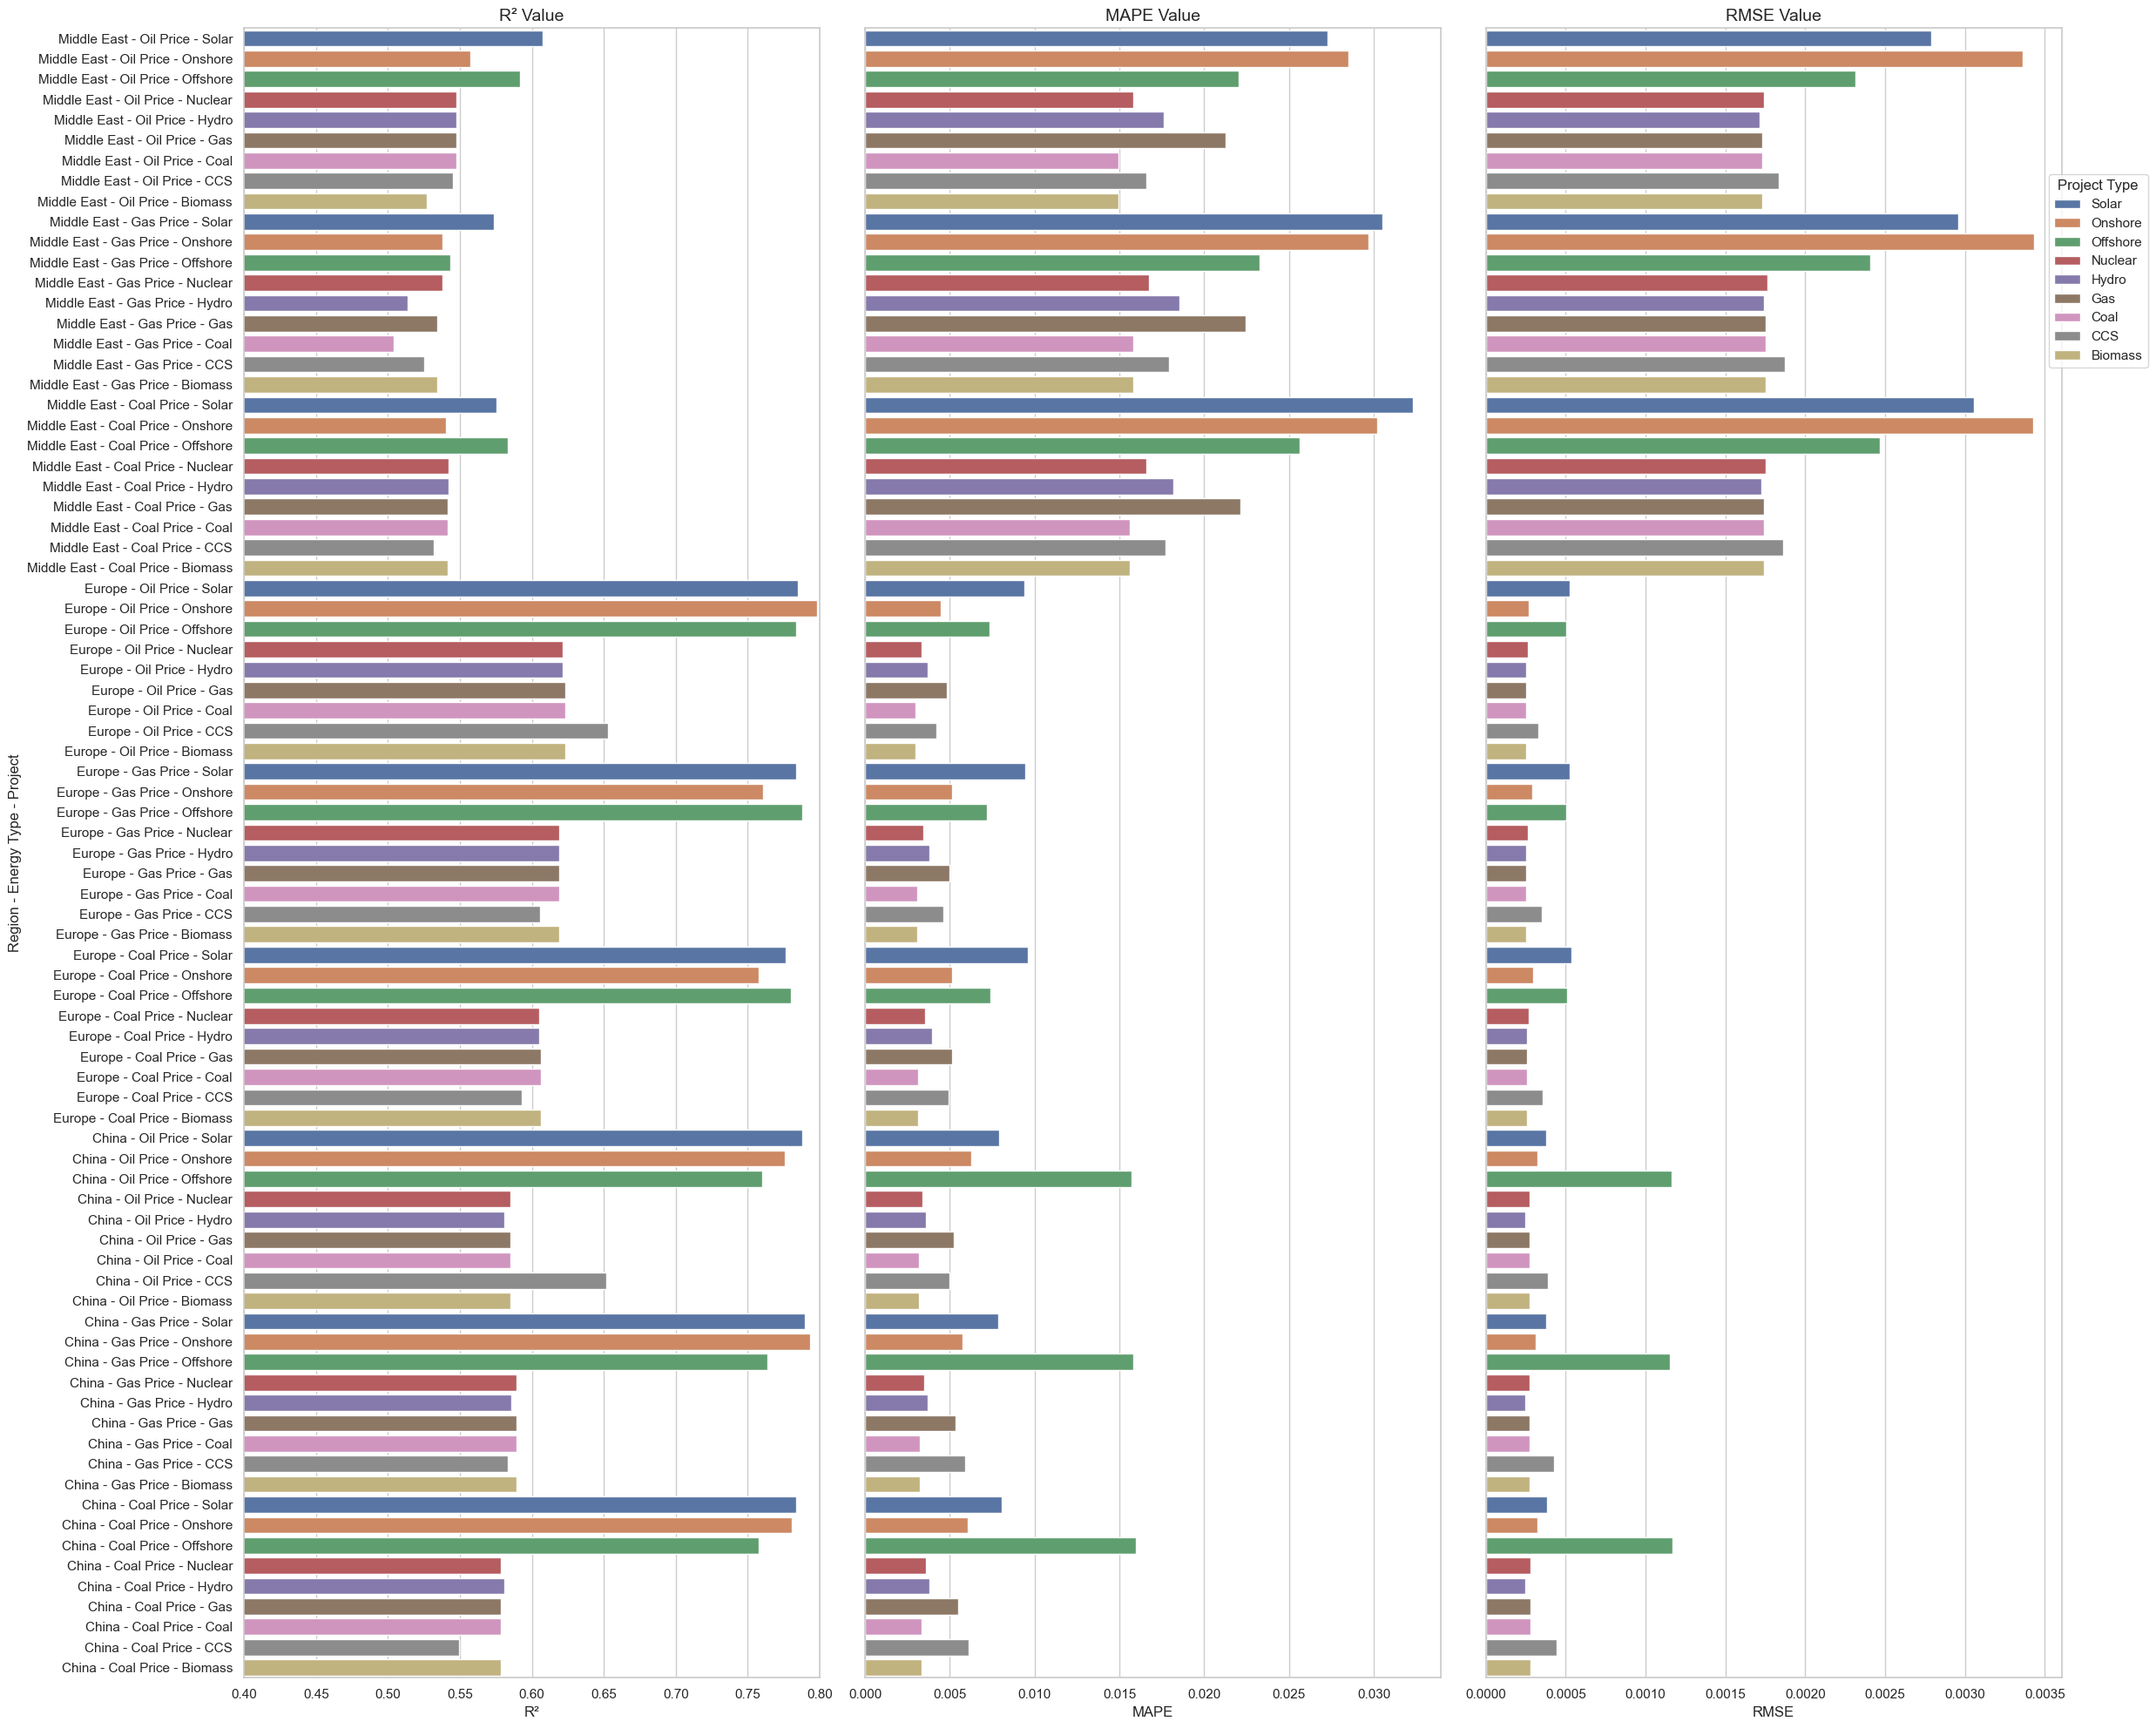
\includegraphics[width=0.98\textwidth]{figure.png}
    \caption{In-sample model performance for each project: comparison of $R^2$, MAPE, and RMSE for estimating WACC across various regions and energy transition projects.}
    \label{fig:result9}
\end{figure*}

\section{Results}

As shown in Fig.~\ref{fig:result9}, the experiment results demonstrate differences in WACC model fit across energy transition projects. Solar and wind (both onshore and offshore) projects demonstrate the highest model fit, with average $R^2$ values all exceeding 0.7. In contrast, other projects, including hydropower, biomass, and coal, exhibit lower model fit, with average $R^2$ values around 0.58.

From a regional perspective, model fit exhibits clear geographical characteristics. In major energy-importing regions like Europe and China, the model fit is higher, with average $R^2$ values of 0.67 and 0.65. Conversely, the model fit is lower in the Middle East, an energy-exporting region, where the average $R^2$ value is 0.55. This disparity is also reflected in the prediction error, as the Middle East's average MAPE (0.0209) is substantially higher than that of Europe (0.0050) and China (0.0061), indicating larger relative prediction errors.

\subsection{Robustness Checks}

The additional holdout and rolling-origin checks support a more cautious interpretation of these results. The main results in Fig.~\ref{fig:result9} summarize in-sample fit within the constructed 2026-2035 panel, while the time-split tests examine how stable the fitted relationships remain when later years are held out. The fixed holdout uses 2026-01 to 2032-12 as the training period and 2033-01 to 2035-12 as the test period. Rolling-origin validation trains through one calendar year and tests the following year.

Across these checks, MAPE remains small for level and trend specifications, but $R^2$ is often unstable because the test-period WACC variation is narrow. Therefore, the paper treats the estimated relationships as predictive sensitivity and stress-scenario evidence rather than as formal causal effects. Table~\ref{tab:robustness} summarizes how the robustness outputs are used in interpreting the findings.

\begin{table}[t]
\centering
\caption{Robustness Checks Used for Interpretation}
\label{tab:robustness}
\scriptsize
\begin{tabular}{P{0.27\linewidth}P{0.30\linewidth}P{0.34\linewidth}}
\toprule
\textbf{Check} & \textbf{Setup} & \textbf{Interpretation} \\
\midrule
Fixed holdout & Train 2026-2032; test 2033-2035 & Later-year prediction is sensitive to specification; use the main $R^2$ values as scenario-fit evidence. \\
Rolling origin & Train through one year; test the next year & Percentage errors are small in level/trend specifications, but $R^2$ varies under narrow WACC ranges. \\
Incremental $R^2$ & Add fuel price and inflation beyond time trend & Positive cases occur for 8/27 China models, 6/27 Europe models, and 6/27 Middle East models (Ridge specifications). \\
Elasticity checks & Log-linear 10\% price shock conversion & Coefficients are interpreted as price-shock sensitivity, not causal effects. \\
\bottomrule
\end{tabular}
\end{table}
